\documentclass[11pt]{article}
\usepackage[utf8]{inputenc}
\usepackage[T1]{fontenc}
\usepackage{graphicx}
\usepackage{booktabs}
\usepackage{amsmath,amssymb}
\usepackage{authblk}
\usepackage[margin=1in]{geometry}
\usepackage[numbers,sort&compress]{natbib}
\usepackage[hidelinks]{hyperref}

\title{Precision@$k$ Is a Great Target and a Dangerous Judge:\\
Model Selection for Fixed-Budget Top-$k$ Problems}
\author[1]{Alejandro G\'omez Ruiz}
\affil[1]{Getronics \\ \texttt{alejandro.gomez@getronics.com}}
\date{\today}

\begin{document}
\maketitle

\begin{abstract}
In many operational problems --- energy-fraud inspection, tax audits, retention
campaigns, medical call-backs --- a model ranks a population and a team acts only on the
top $k$, where $k$ is a fixed external budget. The natural objective is
\emph{precision@$k$}. It is well known that precision@$k$ cannot serve as a training loss
because it is piecewise-constant and non-differentiable; we make the mechanism concrete
with a worked gradient-boosting step. We then ask a less-examined question: should
precision@$k$ be the metric used for \emph{model selection}? Across 93 imbalanced datasets
(90 real, 3 synthetic) with the budget $K$ swept over two orders of magnitude, we find that
selecting a model by validation precision@$k$ yields \emph{significantly worse} held-out
precision@$k$ than selecting by log-loss or average precision (paired Wilcoxon,
$p<2\times10^{-3}$, $n=322$): optimizing selection for the exact target metric is a
losing move, a manifestation of selection-induced optimism (the winner's curse). We
further show that selection difficulty is governed \emph{not} by any scale-free ratio such
as $n_{\text{pos}}/K$ (Spearman $|\rho|\!\approx\!0.19$), but by the absolute
\emph{count} of true positives that land in the budget ($|\rho|\!\approx\!0.43$); its
model-free proxy $\min(K, n_{\text{pos}})$, knowable before training, tracks that count
almost perfectly ($\rho\!=\!0.94$). We give practical recommendations and release all code.
\end{abstract}

\section{Introduction}
Consider a utility's fraud unit whose crew can inspect a fixed number of installations per
month. A meter ranked below the cutoff is never inspected, so calibration or ranking
quality in the bulk of the distribution is operationally irrelevant; only the composition
of the top $k$ matters. We call this a \emph{fixed-budget top-$k$ problem}: score a
population, act on the top $k$, where $k$ is imposed from outside the model (crew size,
budget, legal quota). The natural success metric is
\begin{equation}
\text{precision@}k = \frac{\#\{\text{true positives among the top-}k\text{ scored items}\}}{k}.
\end{equation}
Such problems are ubiquitous (audits, marketing, triage, moderation, lead scoring).

This paper makes three contributions. (i) We give a concrete, per-example account of why
precision@$k$ cannot be a training loss for gradient-based learners
(Section~\ref{sec:loss}). (ii) We show empirically, over 93 datasets, that precision@$k$ is
also a poor \emph{model-selection} metric: log-loss and average precision select
significantly better models on the very precision@$k$ objective
(Section~\ref{sec:results}). This is an instance of the model-selection overfitting studied
by \citet{cawley2010overfitting} and \citet{varma2006bias}, specialised to a high-variance
top-$k$ metric. (iii) We characterise \emph{what} governs the choice: not a ratio of rates
but the absolute number of positives inside the budget, whose a-priori proxy is
$\min(K, n_{\text{pos}})$.

\section{Why precision@$k$ cannot be a training loss}\label{sec:loss}
Precision@$k$ depends on the scores only through the \emph{set} of top-$k$ items. An
infinitesimal change to any single score almost never changes that set, so the metric is
locally constant and its gradient is zero almost everywhere; it changes only at
measure-zero boundaries where two items swap across the cutoff, in jumps of $1/k$
(Fig.~\ref{fig:step}). Gradient boosting fits each new tree to the negative gradient of the
loss (the pseudo-residuals); with precision@$k$ every pseudo-residual is zero, so the
ensemble never moves.

\begin{figure}[h]
\centering

\includegraphics[width=0.95\linewidth]{figs/fig1_step_function.png}
\caption{Sliding one item's score: precision@$k$ is piecewise-constant with a single
cliff (gradient $0$ almost everywhere), whereas log-loss is smooth with an informative
gradient.}
\label{fig:step}
\end{figure}

Table~\ref{tab:grad} makes it concrete for $k=3$. For log-loss with a sigmoid, the gradient
w.r.t.\ each logit is $p-y$: false positives ranked high get large positive gradients
(``push down''), missed positives get negative gradients (``push up''). Every row receives a
signed instruction. Precision@3, by contrast, gives zero for every row: the only helpful
move (lifting $D$ above $C$, changing the top-3 to $\{A,B,D\}$ and precision@3 from
$1/3$ to $2/3$) is a \emph{finite} jump the gradient cannot see. Differentiable surrogates
for top-$k$ losses exist \citep{boyd2012accuracy,kar2015surrogate}, as does the LambdaMART
device of \emph{defining} metric-aware gradients \citep{burges2010ranknet}; for most systems
the pragmatic recipe remains: train on log-loss, evaluate on precision@$k$.

\begin{table}[h]
\centering
\caption{One boosting step, budget $k=3$. Top-3 by score are $A,B,C$, so
precision@3 $=1/3$. Log-loss gradient $=p-y$; precision@3 gradient $=0$ everywhere.}
\label{tab:grad}
\begin{tabular}{ccccc}
\toprule
item & score $p$ & label $y$ & log-loss grad.\ $(p-y)$ & precision@3 grad.\ \\
\midrule
A & 0.92 & fraud (1) & $-0.08$ & 0 \\
B & 0.85 & legit (0) & $+0.85$ & 0 \\
C & 0.80 & legit (0) & $+0.80$ & 0 \\
D & 0.78 & fraud (1) & $-0.22$ & 0 \\
E & 0.60 & fraud (1) & $-0.40$ & 0 \\
F & 0.55 & legit (0) & $+0.55$ & 0 \\
G & 0.30 & fraud (1) & $-0.70$ & 0 \\
H & 0.10 & legit (0) & $+0.10$ & 0 \\
\bottomrule
\end{tabular}
\end{table}

\begin{figure}[h]
\centering
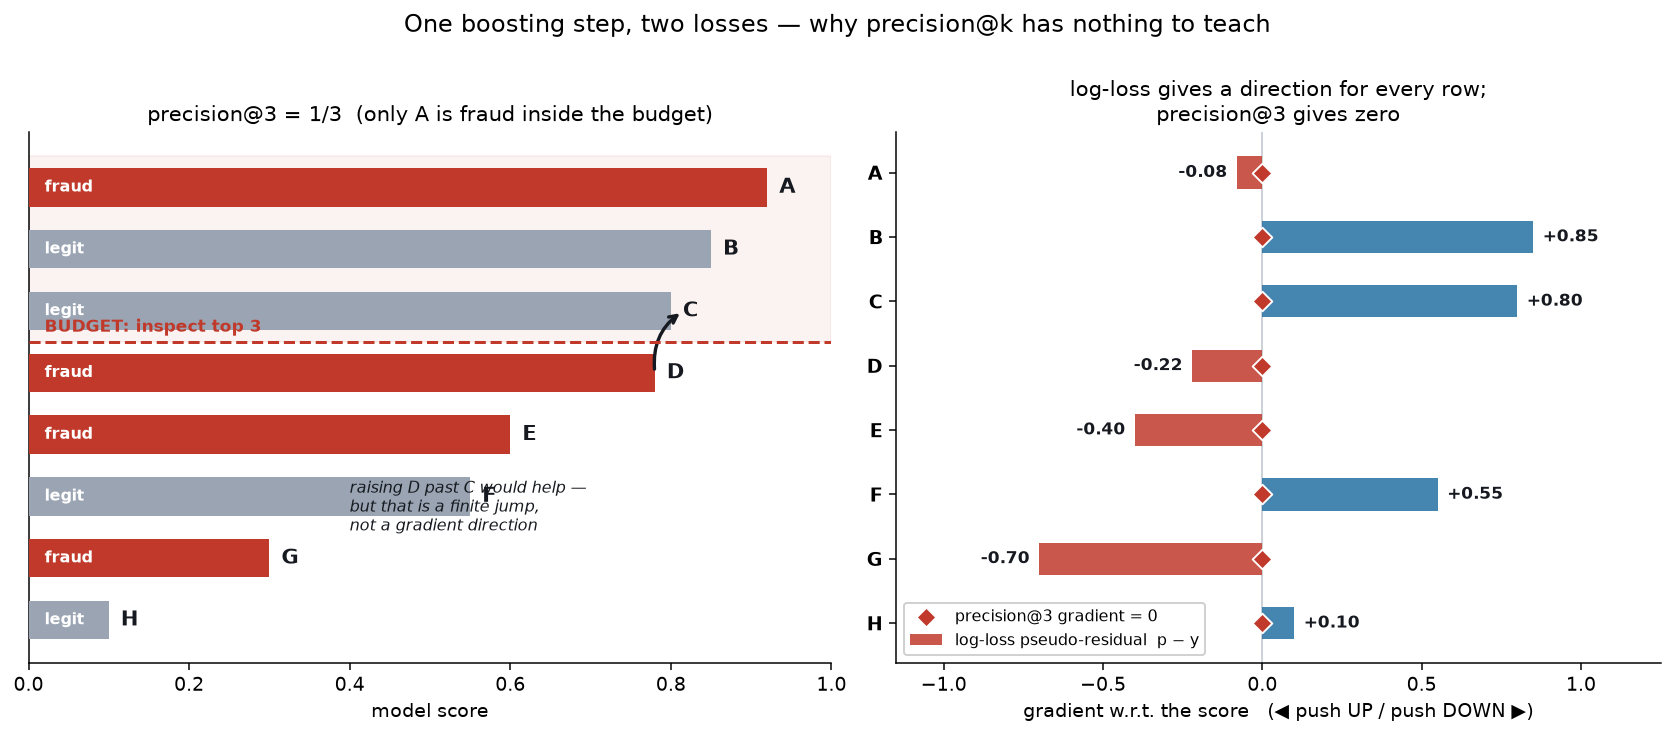
\includegraphics[width=0.95\linewidth]{figs/fig_gradient_example.png}
\caption{The same step visualised. Right: log-loss assigns a direction to every row;
precision@3 assigns zero. Note log-loss already pushes $C$ down and $D$ up --- the swap
that would raise precision@3.}
\label{fig:grad}
\end{figure}

\section{Precision@$k$ as a selection metric: two opposing forces}\label{sec:selection}
Evaluation --- early stopping and choosing among trained configurations --- only requires
\emph{computing} the metric, so precision@$k$ is admissible there. Two forces pull in
opposite directions.

\paragraph{Alignment (favouring precision@$k$).} Log-loss is a global objective: it rewards
calibration across the whole distribution, not the top-$k$ composition. A model can lower
average log-loss by improving many mid-ranked cases while letting a few clear positives slip
out of the budget --- better by log-loss, worse at the operational objective. Only
precision@$k$ detects this.

\paragraph{Stability (against precision@$k$).} Precision@$k$ is a proportion estimated from
$k$ items; its sampling variance is large. Selecting the maximum over many configurations on
one validation set then partly selects noise --- the winner's curse
\citep{cawley2010overfitting} --- so the chosen model generalises worse and the reported
number is optimistically biased. Which force dominates is an empirical question.

\section{Experimental protocol}\label{sec:protocol}
\textbf{Datasets.} 90 real binary imbalanced datasets --- the full \texttt{imbalanced-learn}
benchmark \citep{lemaitre2017imblearn} plus a de-duplicated pull from OpenML
\citep{vanschoren2014openml} (fraud, credit default, software-defect, churn, bankruptcy,
medical screening, satellite/pulsar anomalies), positive rates from $35\%$ to $0.7\%$ ---
plus 3 synthetic datasets. Large sets are subsampled to $30$k rows.

\textbf{Model bank.} Per dataset we split $50/25/25$ (train/validation/test, stratified) and
train $C=40$ LightGBM \citep{ke2017lightgbm} configurations with random hyperparameters, all
on log-loss (scikit-learn tooling \citep{pedregosa2011scikit}).

\textbf{Budget sweep.} We set $K$ to hit target ratios $n_{\text{pos}}/K \in
\{0.25,0.5,1,2,4,8,16\}$, spanning budgets far larger and far smaller than the positive pool.

\textbf{Selection under noise.} We bootstrap \citep{efron1994bootstrap} the validation set
$120$ times; for each metric $m \in \{$precision@$k$, average precision (AP)
\citep{davis2006prroc}, ROC-AUC, log-loss$\}$ we select $\arg\max_c m$ and record that
configuration's \emph{true} quality, precision@$k$ on the held-out test pool.

\textbf{Normalized regret.} To pool heterogeneous datasets we report, per (dataset, $K$),
\begin{equation}
\mathrm{regret}(m) = \frac{q^\star - \bar q_m}{q^\star - \bar q_{\text{avg}}},
\end{equation}
where $q^\star$ is the best test precision@$k$ in the bank (oracle), $\bar q_m$ the mean test
quality selected by $m$, and $\bar q_{\text{avg}}$ the average model's quality. $0$ means
oracle selection, $1$ means no better than picking at random. We keep the $322$ (of $625$)
cases with a non-trivial gap ($q^\star-\bar q_{\text{avg}}\ge 0.02$). Following
\citet{demsar2006statistical} we compare metrics with the paired Wilcoxon signed-rank test.

\section{Results}\label{sec:results}

\paragraph{Log-loss and AP beat precision@$k$, significantly.}
Table~\ref{tab:main} and Fig.~\ref{fig:overall} summarise the pooled comparison. Log-loss and
AP tie for the lowest mean regret and are statistically indistinguishable from each other
($p=0.53$); each beats precision@$k$ with $p<2\times10^{-3}$. AUC is no better than
precision@$k$ ($p=0.85$). In words: \emph{selecting on the metric you ultimately care about
gives you a worse model, on that same metric, than selecting on a more stable proxy.}

\begin{table}[h]
\centering
\caption{Model-selection metrics pooled over $322$ (dataset, budget) cases. Mean normalized
regret (lower is better), win-rate (fraction of cases where the metric picked the single best
model), and paired Wilcoxon $p$-value versus precision@$k$.}
\label{tab:main}
\begin{tabular}{lccc}
\toprule
selection metric & mean regret $\downarrow$ & win-rate & Wilcoxon $p$ vs.\ P@$k$ \\
\midrule
log-loss          & \textbf{0.714} & \textbf{34\%} & $6.1\times10^{-4}$ \\
average precision & 0.719 & 21\% & $1.2\times10^{-3}$ \\
ROC-AUC           & 0.770 & 20\% & $0.85$ (n.s.) \\
precision@$k$     & 0.790 & 25\% & --- \\
\bottomrule
\end{tabular}
\end{table}

\begin{figure}[h]
\centering
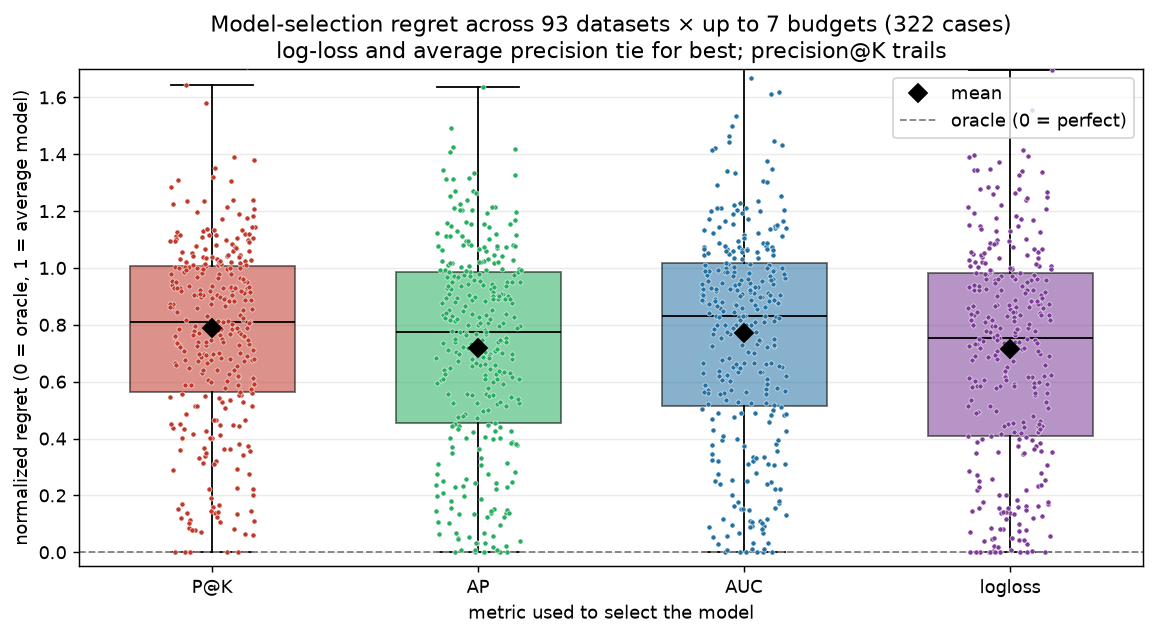
\includegraphics[width=0.85\linewidth]{figs/figT0_overall.png}
\caption{Distribution of normalized regret per selection metric across the $322$ cases;
diamonds mark means. Log-loss and average precision lead; precision@$k$ trails.}
\label{fig:overall}
\end{figure}

\paragraph{It is a count, not a ratio.}
One might expect precision@$k$ to be safe whenever the budget is large relative to the
positives (large $n_{\text{pos}}/K$). It is not: that ratio barely orders regret
(Spearman $|\rho|=0.19$). What orders it is the \emph{absolute number of true positives inside
the budget} ($\approx$ precision $\times\,K$; $|\rho|=0.43$), Fig.~\ref{fig:count}. A
proportion's reliability is set by the number of successes behind it --- a count, not a
fraction --- so two problems with the same ratio behave differently if one is ten times
larger.

\begin{figure}[h]
\centering
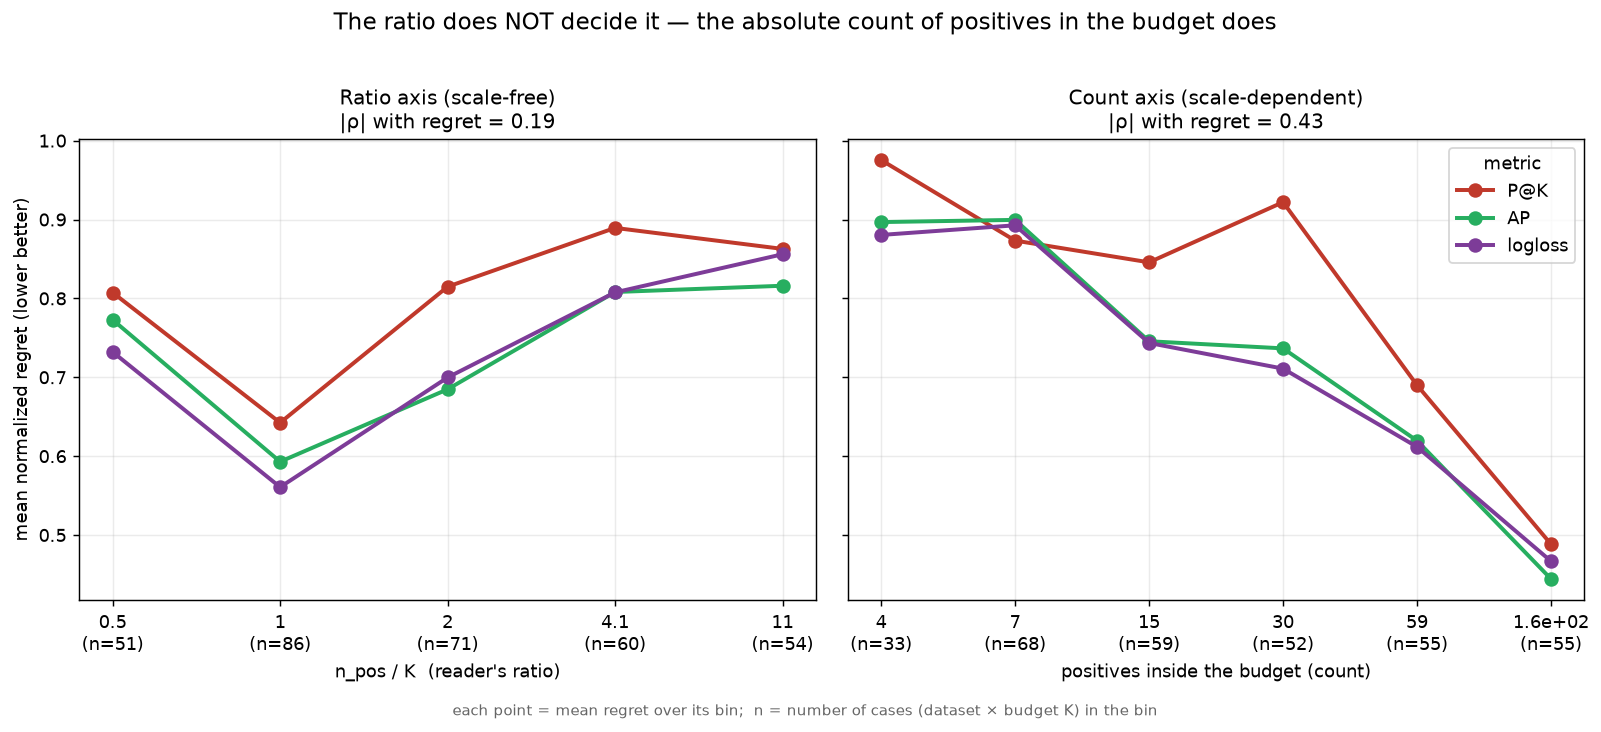
\includegraphics[width=0.98\linewidth]{figs/figT2_ratio_vs_count.png}
\caption{Left: the scale-free ratio $n_{\text{pos}}/K$ barely orders regret. Right: the
absolute count of positives inside the budget does. $n$ = number of (dataset, budget) cases
per bin.}
\label{fig:count}
\end{figure}

\paragraph{The count is knowable a priori.}
The achieved count (precision $\times\,K$) depends on the model, but its model-free upper
bound $\min(K, n_{\text{pos}})$ --- the most positives that could possibly land in the budget
--- predicts almost as well ($|\rho|=0.38$) and tracks the achieved count almost perfectly
($\rho=0.94$), Fig.~\ref{fig:apriori}. So the deciding quantity is available before training;
for the exact value, count the true positives in a single cheap baseline's top-$k$.

\begin{figure}[h]
\centering
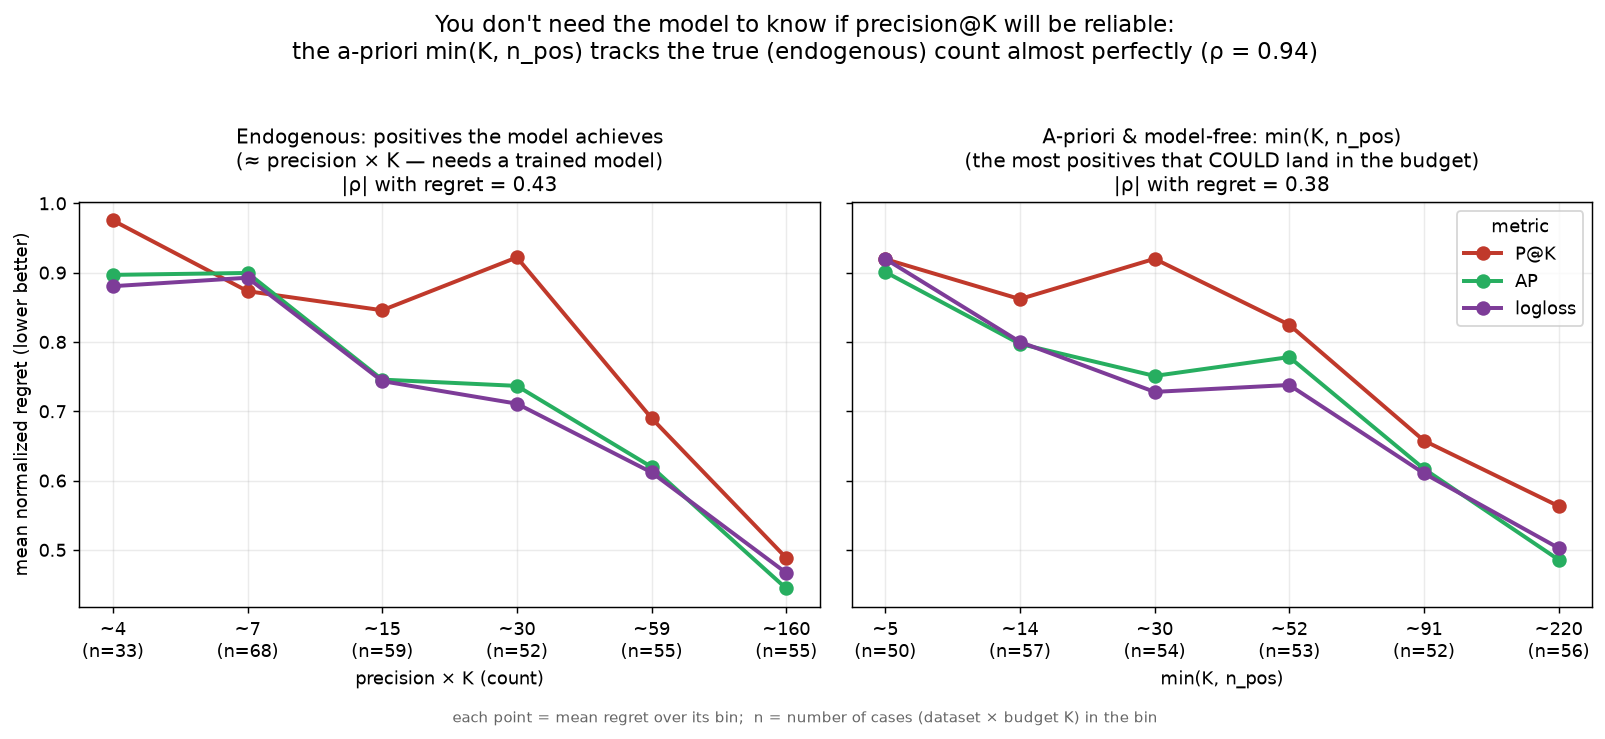
\includegraphics[width=0.98\linewidth]{figs/figT6_apriori.png}
\caption{The endogenous count precision $\times\,K$ (left) and its a-priori, model-free proxy
$\min(K, n_{\text{pos}})$ (right) order regret almost identically ($\rho=0.94$ between them).}
\label{fig:apriori}
\end{figure}

\paragraph{The reported number is inflated too.}
Consistent with the winner's curse, validation precision@$k$ overstates true precision in
proportion to how few positives sit in the budget --- by tens of percent, occasionally more
than $2\times$ --- so it is also an optimistic estimate of production performance
(Fig.~\ref{fig:opt}).

\begin{figure}[h]
\centering
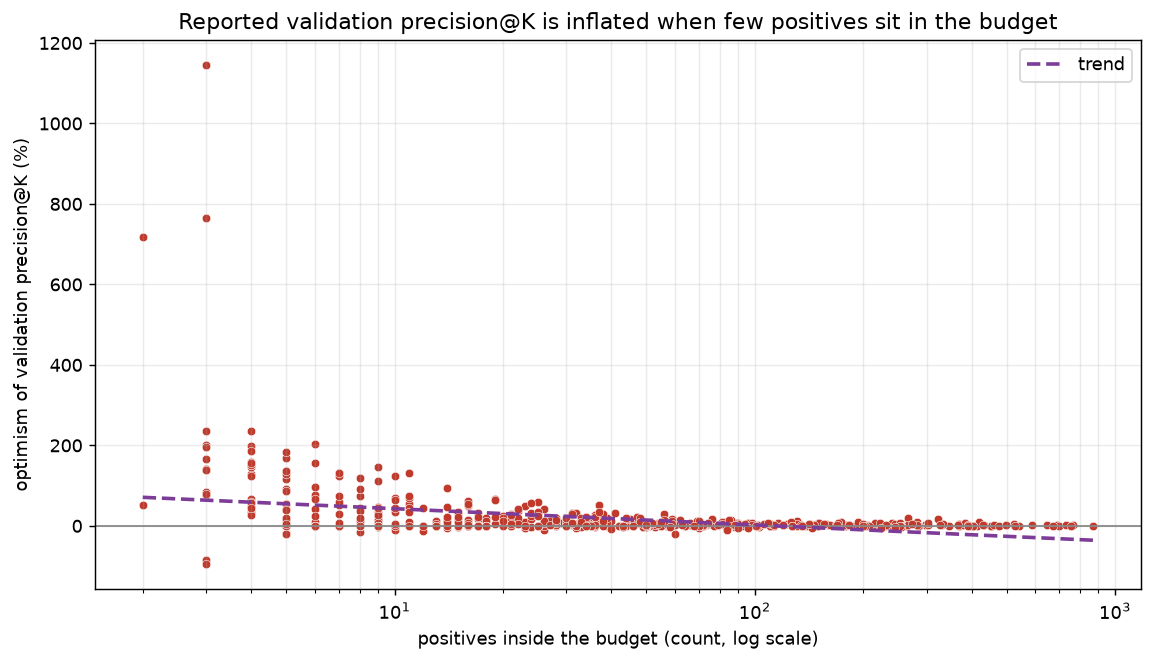
\includegraphics[width=0.8\linewidth]{figs/figT5_optimism.png}
\caption{Optimism of validation precision@$k$ (over-statement of the selected model's true
precision) versus the number of positives in the budget.}
\label{fig:opt}
\end{figure}

\section{Discussion and recommendations}
Keep precision@$k$ as the target and the headline evaluation metric, but not as the training
loss and not, by default, as the selection metric. For selection, \textbf{default to average
precision or log-loss}; use precision@$k$ only as a tie-breaker. The single lever that
matters is knowable in advance: $\min(K, n_{\text{pos}})$, the number of positives that can
land in the budget. When it is small, no selection metric is reliable --- invest in more
labelled positives or a larger budget, not a cleverer metric. Finally, never quote raw
validation precision@$k$ as expected production performance when the budget is positive-poor;
report a nested/held-out estimate.

\section{Limitations}
We study one model family (LightGBM) and a fixed model bank, isolating selection noise but
not early stopping (where the same variance argument applies). Ground-truth precision@$k$ on
small datasets is itself estimated with noise, mitigated by pooling and by robust statistics
(rank, win-rate, signed-rank tests). Results are statements about \emph{expected} selected
quality. Extending to neural and linear models, and to explicit top-$k$ surrogate training,
is future work.

\section{Conclusion}
The metric you optimize and the metric you select with need not be the same. For fixed-budget
top-$k$ problems, selecting on a stable proxy (log-loss, average precision) beats selecting on
the noisy target metric itself, and the deciding factor is a plain count --- how many
positives your budget will contain --- not a ratio of rates.

\paragraph{Reproducibility.} All code, the dataset list, and figures are released at
\url{https://github.com/USERNAME/precision-at-k-study} and run from a fixed seed.

\bibliographystyle{plainnat}
\bibliography{refs}
\end{document}
